\section{Coverage}
\label{sec:cov}
\textit{The Dean feels that it is not economically justified to by a robot system for 80.000 euro just to collect cups. Hence, it is interesting to have the robot do a second task, namely washing of the floors. Therefore calculate a coverage path that covers most of the floor in the map. Again the robot must start and end at the offloading stations.
Again, you are free to choose algorithm and you should document the choice, the distance in kilometres that the robot moves and how long it takes to compute the coverage path.}


\subsection{Funktioner}

Følgende er en oversigt over relavante funktioner i Coverage delen.

\begin{itemize}
	\item cover\_vertex(goal\_x,goal\_y)
	\begin{itemize}
		\item cup\_scanner()
		\item collect\_cup(location)
	\end{itemize}
	
\end{itemize}

\paragraph{\texttt{cover\_vertex(goal\_x,goal\_y)}}
Robotten vasker en region fra den lokation den befinder sig på, til det punkt der er givet som argument. For hvert skridt den tager, udfører den en komplet skanning efter kopper. Da robotten kan detektere kopper i en radius af to meter, men kun kan samle dem op i en radius af en meter, bliver de detekterede koppers lokation lagt ind i en kø. For hvert skridt robotten tager, checker den om de detekterede kopper i køen er indenfor rækkevidde, hvorefter de kan blive samlet op.

\texttt{cover\_vertex(goal\_x,goal\_y)} kan beskrives som det følgende:
\begin{lstlisting}
while !finished
	scan for cups
		if cup detected
			save to found cups vector
	if found cup is within range && cups in tray < max number of cups
		pick up cup
	if tray is full
		empty cups and return
	switch case:
		walk down 
			if y-goal !reached
				y position++
			else walk from bottom
		walk right from bottom 
			if x-goal !reached&&rightsteps<2xradius
				x position++
			else walk up
		walk up
			if start y !reached
				y position--
			else walk right from top
		walk right from top
			if x-goal !reached&&rightsteps<2xradius
				x position++
			else walk down
	if goal is within reach
		finish=true
\end{lstlisting}


\newpage
\subsection{Resultater}
Figur \ref{fig:res} viser et lille uddrag af dækningsarealet. Det originale kort samt en .gif animation af robottens proces er uploadet.\todo{.gif part 1 og 2 fylder for meget.}
\begin{figure}[th!]
\centering
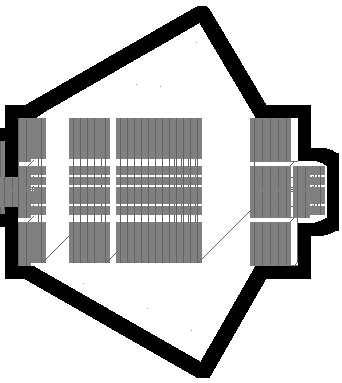
\includegraphics[width=0.5\textwidth]{./graphics/efterVask}
\caption[tekst i indholdsfortegnelsen]{Udsnit af dækningsareal.}
\label{fig:res}
\end{figure}
Den store fordel med den besluttede regionsopdeling er, at den virker rigtig godt for firkantet rum. Hvis rummene derimod ikke er firkantet som set i figur \ref{fig:res}, er regionsopdelingen mindre effektiv. Dette skyldes der dannelse af regioner med intet indvendigt areal. Regioner med intet indvendigt areal vil ikke returnere et af det fire scenarier P\(_{1, 9, 10, 11}\) i \emph{stageTwo()} og herved vil den endelige region ikke blive oprettet.
En måde at løse denne problemstilling på kunne være at implementere en \emph{Bush Fire} algoritme i hvert rum og første gang lad den brænde robottens radius ind fra væggene og herefter lad den brænde robottens diameter indtil hele rummet er "brændt af".


Opsummerende resultater fra part 1 og 2 ses i tabel \ref{tb:resultater}. 

\begin{figure}[th!]
\centering
\begin{tabular}{l|l}
\# & \\\hline
Beregnings tid af regioner & 6,809 s \\
Antal regioner & 4178 stk\\
Beregnings tid af vaks og opsamling af kopper & 8,14 min \\
Antal opsamlet kopper & 267 stk\\
Total distance kørt & 86,37 km\\
Operations tid for robot & 17,27 t
\end{tabular}
\captionsetup{type=table}
\caption[tekst i indholdsfortegnelsen]{Opsummerende resultater fra robotten.}
\label{tb:resultater}
\end{figure}
Som det fremgår af tabel \ref{tb:resultater} tager det knap 7 sekunder at inspicere alle rum og knap 9,5 minut at vaske gulvarealerne. Ligeledes fremgår det at robotten har en total operations tid på 17,27 timer med en hastighed på 5 km/t. 







